\documentclass[A4]{scrartcl}
\usepackage[paper=a4paper,left=10mm,right=10mm,top=25mm,bottom=25mm]{geometry}
\usepackage[utf8]{inputenc}
\usepackage{graphicx}

\begin{document}
  \addsec{Ideale Operationsverstärker}
  Goldene Regeln für gegengekoppelte Verstärker:\\
  1. $I_{in} = 0$ "In die Eingänge fließt kein Strom","Der Eingangswiderstand ist Unendlich"\\
  2. $U_{NIV} = U_{IV} = 0V$ 

  \addsec{Reale Operationsverstärker}
  Bias- und Offsetströme\\
  Offsetspannungen\\
  Kompensationsschaltungen\\

  \addsec{Analoge Rechenschaltungen}
  Impedanzwandler:\\
  Addierer:\\
   -invertierend\\
   -nicht invertierend\\
  Subtrahierer:\\
  Integrierer:\\
  Differenzierer:\\
  Strom-Spannungs-Wandler:\\
  Logarithmierer: (Schreibt man das so ?)\\
  Exponenzierer:\\
  
  \newpage
  \addsec{Filter 1. Ordnung}
  Definitionen:\\
  Ausgangsspannung des TP := $U_A$\\
  Eingangsspannung des TP := $U_E$\\
  Impedanz des Widerstands := $Z_R$\\
  Impedanz des Kondensators := $Z_C$\\
  Kapazität des Kondensators := $C$\\
  Widerstand des Widerstands := $R$\\
  Grenzfrequenz des Filters := $f_c$\\
  \\
  Übertragungsfunktion Tiefpass:\\
  Herleitung:\\ 
  \begin{tabular}{l|l}
    Allgemeiner Zusammenhang Spannungsteiler:& $\frac{U_A}{U_E} = \frac{Z_C}{Z_R+Z_C}$\\
    Einsetzen der Bauteilgleichungen:& $\frac{U_A}{U_E} = \frac{\frac{1}{s\cdot C}}{R + \frac{1}{s \cdot C}}$\\
    Bruch mit $s\cdot C$ erweitern:& $\frac{U_A}{U_E} = \frac{1}{s \cdot RC + 1}$\\
    Einsetzen des Zusammenhangs $\frac{1}{RC} = 2\pi f_c$:& $\frac{U_A}{U_E} = \frac{1}{1 + \frac{s}{2\pi f_c}}$\\
    Einsetzen des Zusammenhangs $s = j2\pi f$ :& $\frac{U_A}{U_E} = \frac{1}{1 + \frac{j2\pi f}{2\pi f_c}}$\\
    Kürzen:& $\frac{U_A}{U_E} = \frac{1}{1 + \frac{jf}{f_c}}$\\
    Übertragungsfunktion Hochpass:\\
    Herleitung:\\ 
    Allgemeiner Zusammenhang Spannungsteiler:& $\frac{U_A}{U_E} = \frac{Z_R}{Z_R+Z_C}$\\
    Einsetzen der Bauteilgleichungen:& $\frac{U_A}{U_E} = \frac{R}{R+\frac{1}{s \cdot C}}$\\
    Bruch mit $\frac{s\cdot C}{s\cdot C}$ erweitern:& $\frac{U_A}{U_E} = \frac{s \cdot RC}{s \cdot RC+1}$\\
    Einsetzen des Zusammenhangs $\frac{1}{RC} = 2\pi f_c$ und Kürzen:& $\frac{U_A}{U_E} = \frac{1}{1+\frac{f_c}{jf}}$\\
  \end{tabular}

  \addsec{Filter höherer Ordnung}
  Übertragungsfunktion TP allg: $G(s) = \frac{A_0}{1+\frac{2D}{\omega_0}s+\frac{1}{\omega_0^2}s^2} = \frac{A_0}{1+a_1 s_n + b_1 s_n^2},s_n = \frac{s}{\omega_c}$ (TODO Überprüfung ob $\omega_0 oder \omega_C$ in 1. Formel)\\
  Dämpfung: $D = \frac{1}{2Q}$\\
  Dämpfung aus Overshoot: $D = \sqrt{\frac{ln^2(os)}{ln(os)^2+\pi^2}}$\\
  Gleichspannungsverstärkung: $A_0 = - \frac{R_2}{R_1}$\\
  Grenzkreisfrequenz: $\omega_c = \sqrt{b_1}\cdot \omega_0$\\
  
  \addsec{Sallen Key Filter}
  Übertragungsfunktion TP: $\frac{U_a}{U_e} = \frac{\alpha}{1+s((1-\alpha)R_1C_2+s^2R_1R_2C_1C_2}, \alpha = A_0$\\
  
  \addsec{Multiple Feedback Filter}
  Übertragungsfunktion TP: $\frac{U_a}{U_e} = \frac{\frac{R2}{R1}}{1+sC_1\cdot (\frac{R_3 R_2}{R_1} + R_2 + R3_3) + s^2C_1C_2R_2R_3 }$\\
  Eigenkreisfrequenz: $\omega_0 = \frac{1}{\sqrt{C_1C_2R_2R_3}}$\\
  Q-Faktor: $Q = \frac{1}{\omega_0 (\frac{R_2R_3}{R_1}+R_2+R3)}$\\
  Amplitudengang: $|A_0(\omega)| = \frac{\frac{R_2}{R_1}}{\sqrt{(1-\frac{\omega}{\omega_0})^2+(2D\frac{\omega}{\omega_o})}}$ (TODO: Testen und Herleiten omega-0 Fraglich)

  \addsec {Schaltungen mit Mitkopplung}
  \addsec {nichtinvertierender Komparator}
  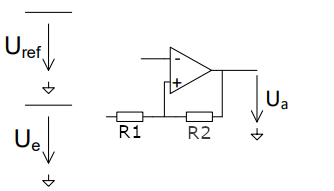
\includegraphics[width=0.33\textwidth]{Komparator.png}
  \addsec {invertierender Komparator}
  \addsec {Fensterkomparator}
  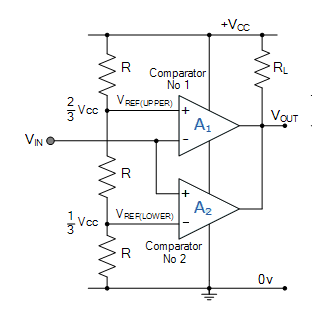
\includegraphics[width=0.33\textwidth]{Fensterkomparator.png}
  \addsec {Rechteck - Dreieckgenerator}
  \addsec {vereinfachter Dreieckgenerator}
  \addsec {PWM Generator}
  
\end{document}
